% !TeX spellcheck = en_GB

\documentclass{article}

\usepackage{amssymb}
\usepackage{rotate}
\usepackage{fancyvrb}
\usepackage[utf8]{inputenc}
\usepackage[small,bf,hang]{caption}
\usepackage{refstyle}
\usepackage[english]{babel}
\usepackage{amsmath}
\usepackage{graphicx}
\usepackage{float}
\usepackage{gensymb}
\usepackage{caption}
\usepackage{subcaption}
\usepackage{parskip}
\usepackage{fancyhdr}
\usepackage{vmargin}
\usepackage{pgf}
\usepackage{float}
\usepackage{pdfpages}
\usepackage{mathtools}
\usepackage{gensymb} %\degree
\usepackage{hyperref}
\usepackage{color}
\usepackage[export]{adjustbox}%\includegraphics[,left/center/right]{imagefile}%can also be done by \raggedright/\centering
%\usepackage{showframe}
\usepackage[colorinlistoftodos]{todonotes}



\newcommand{\hoek}[1]{{#1}^{\circ}}

\hypersetup{
	colorlinks=true, % make the links colored
	linkcolor=black, % color TOC links in blue
	urlcolor=black, % color URLs in red
	linktoc=all % 'all' will create links for everything in the TOC
}

\title{Project 1: \\ Autonomous vehicle for package storage}								% Title
%\author{Shelly De Sutter}
%\author{Ayoub El Moussaoui}				
%\author{Fabrice Mutabazi}
%\author{Jeroen Taets}
%\author{Gilke Van Hove}
\date{\today}											% Date

\makeatletter
\let\thetitle\@title
\let\theauthor\@author
\let\thedate\@date
\makeatother

\pagestyle{fancy}
\fancyhf{}
\lhead{\textsc{\thetitle}}
\cfoot{\thepage}
\graphicspath{{Figures/}{}}

%\pdfminorversion=9
%\pdfobjcompresslevel=9
%\pdfcompresslevel=9

\begin{document}
	%	\listoftodos
	\begin{titlepage}
		\raisebox{0 cm}[0pt][0pt]{%
			\makebox[\textwidth][l]{\includegraphics[scale=1]{UGent}\hfill\includegraphics[scale=1]{UGent_EA}}}\\[5 cm]
		%\begin{figure}
		%\raggedright
		%\includegraphics[scale=7]{UGent}
		%\end{figure}
		\centering
		\Large GHENT UNIVERSITY, ICT \& MECHATRONICS COURSE\\
		\vspace*{0.5 cm}
		%\includegraphics[scale = 0.15]{Ghent_University_logo}\\[1.0 cm]	% University Logo
		\textsc{\large }\\[0.5 cm]			% Course Name
		\rule{\linewidth}{0.2 mm} \\[0.4 cm]
		{\Large \bfseries \thetitle \\ Final report}\\
		\rule{\linewidth}{0.2 mm} \\[1.5 cm]
		\textsc{\normalsize}\\[0.5cm]
		\begin{center} \large
			\emph{Group 1A:}\\
			\Large Matthias De Hantsetters\\
			\Large Jonathan Deschodt\\
			\Large Reinout Lavens\\
			\Large Jonas Vanheule\\
			
			\vspace*{0.5 cm}
			\Large Supervisors: \\ Prof. dr. ir. Frederik De Belie \& Ir. Wannes De Groote\\ 
			
		\end{center} ~		
		\vfill
		{\Large Academic year 2018-2019}\\[2 cm]
		
		\vfill
		
	\end{titlepage}
	
	\tableofcontents
	\pagebreak
	\pagenumbering{arabic}
	
	\section{Introduction}
	\par In this project a robot is designed, able to stack blocks in a specified order, based on their colour. The project assignment prescribes several stacking strategies e.g. four blocks with each a unique colour, will be placed on three positions and need to be stacked in a predetermined order on a fourth position. The dimensions of the blocks are 4cm x 4cm x 4cm and placed 4cm apart. Since the stacking of several blocks is required, accurate positioning is of high importance. Moreover the use of the colour sensor in different conditions requires some attention.
	\par The robot is built using the LEGO Mindstorms eduction set with the EV3 intelligent brick as the heart and brain. Three motors, a colour sensor and some ultrasonic sensors were available. 
	
	\section{Objectives}
	\par The goal of this project is the design and construction of a palletizing robot capable of stacking
	4 cubes (with the same dimensions but different colours) on top of each other in a certain
	colour order. The gripping mechanism must be mechanical without the involvement of magnets
	and should only be able to pick up 1 cube at a time. The focus of the project will be on
	the actuation and positioning of the gripper, as well as the stacking/sorting algorithm to get
	the cubes in their correct stacking order. The blocks will initially be placed at predefined, linear
	and equidistant positions. The top of the bill will be playing a Tower of Hanoi game.
	
	\section{Mechanical design}
	\begin{figure}[H]
		\centering
		\includegraphics[keepaspectratio, width=\textwidth]{Figures/Mechanical_Structure.jpg}
		\caption{Mechanical structure}
		\label{fig:Mechanical}	
	\end{figure}
	
	
	\par The robot has to stack blocks placed initially on a straight line, therefore the robot drives on the floor guided by rails to avoid deflection. The wheels are driven by a large motor. The lifting mechanism is executed by a caterpillar track, which carries the gripper. A difficulty was tightening the track for less vibration. The caterpillar track is also driven by a large motor, while the gripper by a medium. A colour sensor is placed in the middle of the gripper. It is necessary that the blocks are close to the sensor since the colour sensor only works within a range of a few centimeters. Since the colour sensor is attached to the gripper, only the upper block of a stack can be seen. In addition, two ultrasonic sensors are mounted on the robot.
	
	\par Due to poor reliability of the ultrasonic sensors in certain ranges, they are both used in homing reference. The first sensor measures the horizontal distance from the reference to a certain homing position, further movement are then achieved by use of the motor encoder (further also mentioned as the softwarematic 'tachocounter'). The same is true for the second sensor, which is placed at the back of the caterpillar and measures the vertical distance of the gripper to the floor. It too is used only during the calibration sequence of the gripper vertical motion. Both these movement can be achieved by the tachocounter due to the rigidity of the wheel and the caterpillar transmission, the latter being more rigid and achieving a better precision. 
	
	\par The EV3 intelligent brick is the heaviest part and is used as counterweight since the gripper at the highest position tilts the robot. The supporting rope, as seen on Figure \ref{fig:Mechanical}, ensures that the sensor doesn't hang down at the lowest position, due to the flexibility of the caterpillar.
	
	\section{Sensing}
	\par As mentioned above, several sensors are attached to the robot. Although it ensures flexibility and robustness, in big projects it comes literally with a cost. Therefore also this project deals with the challenge to avoid additional sensors, if it is possible, and in meantime to ensure the performance of indirect sensing. 
	
	\par In this project there is positioning and colour-sensing. More specific, the positioning consists of homing, get an actual position, get a height detection of the stacks and detect clamping of the gripper. Obviously the colour-sensing consists of recognizing a predetermined colour.
	
	\subsection{Position-sensing}
	\subsubsection{Horizontal movement}
	\par If the amount of resources is unlimited, the absolute ultrasonic distance sensors are a perfect match. Ideally, even homing and calibration is not necessary. Unless in reality, they deal with some problems.
	
	\par In a first approach, the sidewards movement is equipped with one of those ultrasonic sensors. The sensor provides an absolute distance independently of the flexible connection between tires and the ground. Therefore a closed loop control with the ultrasonic sensor and the large motor is developed. Two problems revealed during testing these strategy. First, in a superficial approach the sensor had a likely linear behaviour with respect to the effective distance. Despite this, a more thorough investigation (Figure \ref{fig:Cal_ultrasonic}) delivers a non-linear behaviour around the stacking environment of stack 2 and 3. Second, closing the control loop is not straightforward as thought. Since the Lejos motors have a tachocounter-based PID control loop deep in the code, it's not easy to create a similar closed loop control on the higher coding level or to replace the tachocounter by the ultrasonic sensor in the deeper code. Moreover, due to the used ICT-structure (Blackboard), an uncertain delay between the obtained sensor values and the control loop is detrimental for smooth accurate performance. In following paragraphs, these problems and their solutions are explained in detail.
	
	\begin{figure}[H]
		\centering
		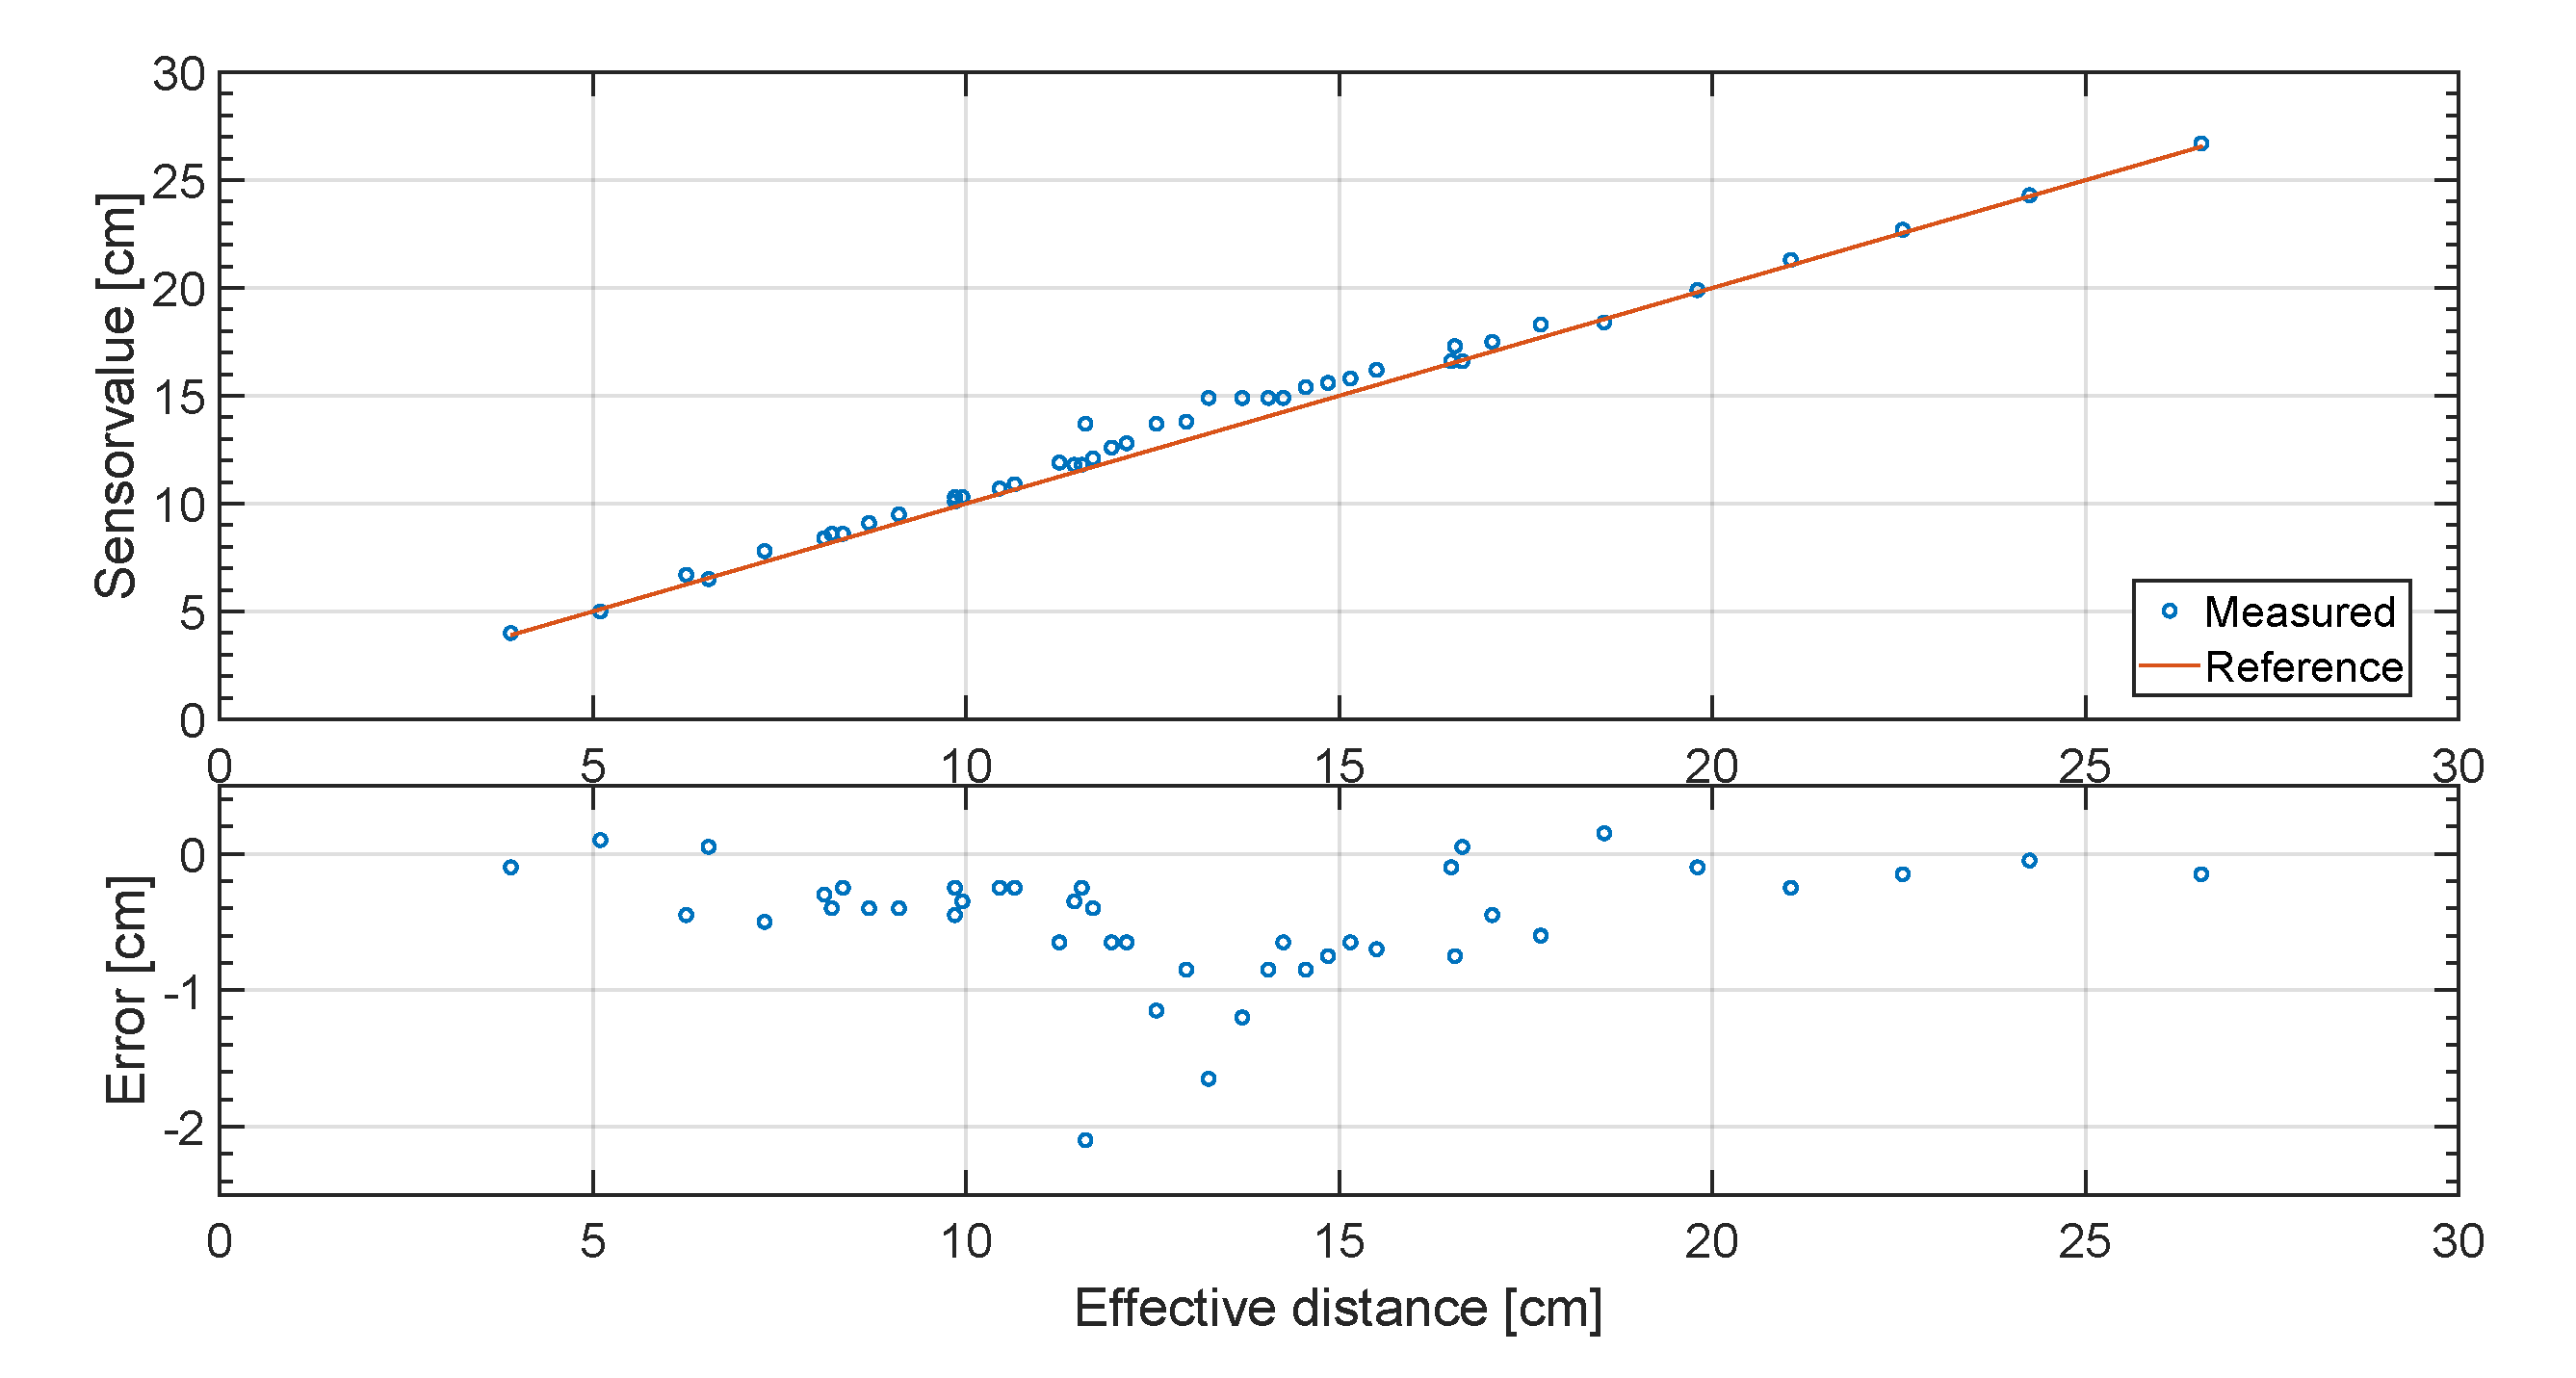
\includegraphics[keepaspectratio, width=\textwidth]{Figures/UltraSoon_XPos_Cal_Curve.pdf}
		\caption{Static measurement of the ultrasonic sensor in the x-direction.}
		\label{fig:Cal_ultrasonic}
	\end{figure}
	
	\par Non-linearity has been mapped by static measurements (Figure \ref{fig:Cal_ultrasonic}). The measurement imparts two conclusions. First, once the robot is at a certain location, the value of the sensor is steady. If the robot is pulled out of that position and pulled in again, the value could vary. Hence the conclusion that the sensor has hysteresis and its sensor value has a certain probability. On the other hand, there is a slight pattern in the measured curve. The divergence increases towards 13 cm (effective distance) and decreases afterwards. This effect is assigned to a steady non-linearity curve. The latter could easily be resolved by implementing a calibration curve into the controller. How the former will be dealt with is not straightforward. On top of that, the obtained measurements are at stand-still, while the sensor is used while moving, which implies additional uncertainties. 
	
	\begin{figure}[H]
		\centering
		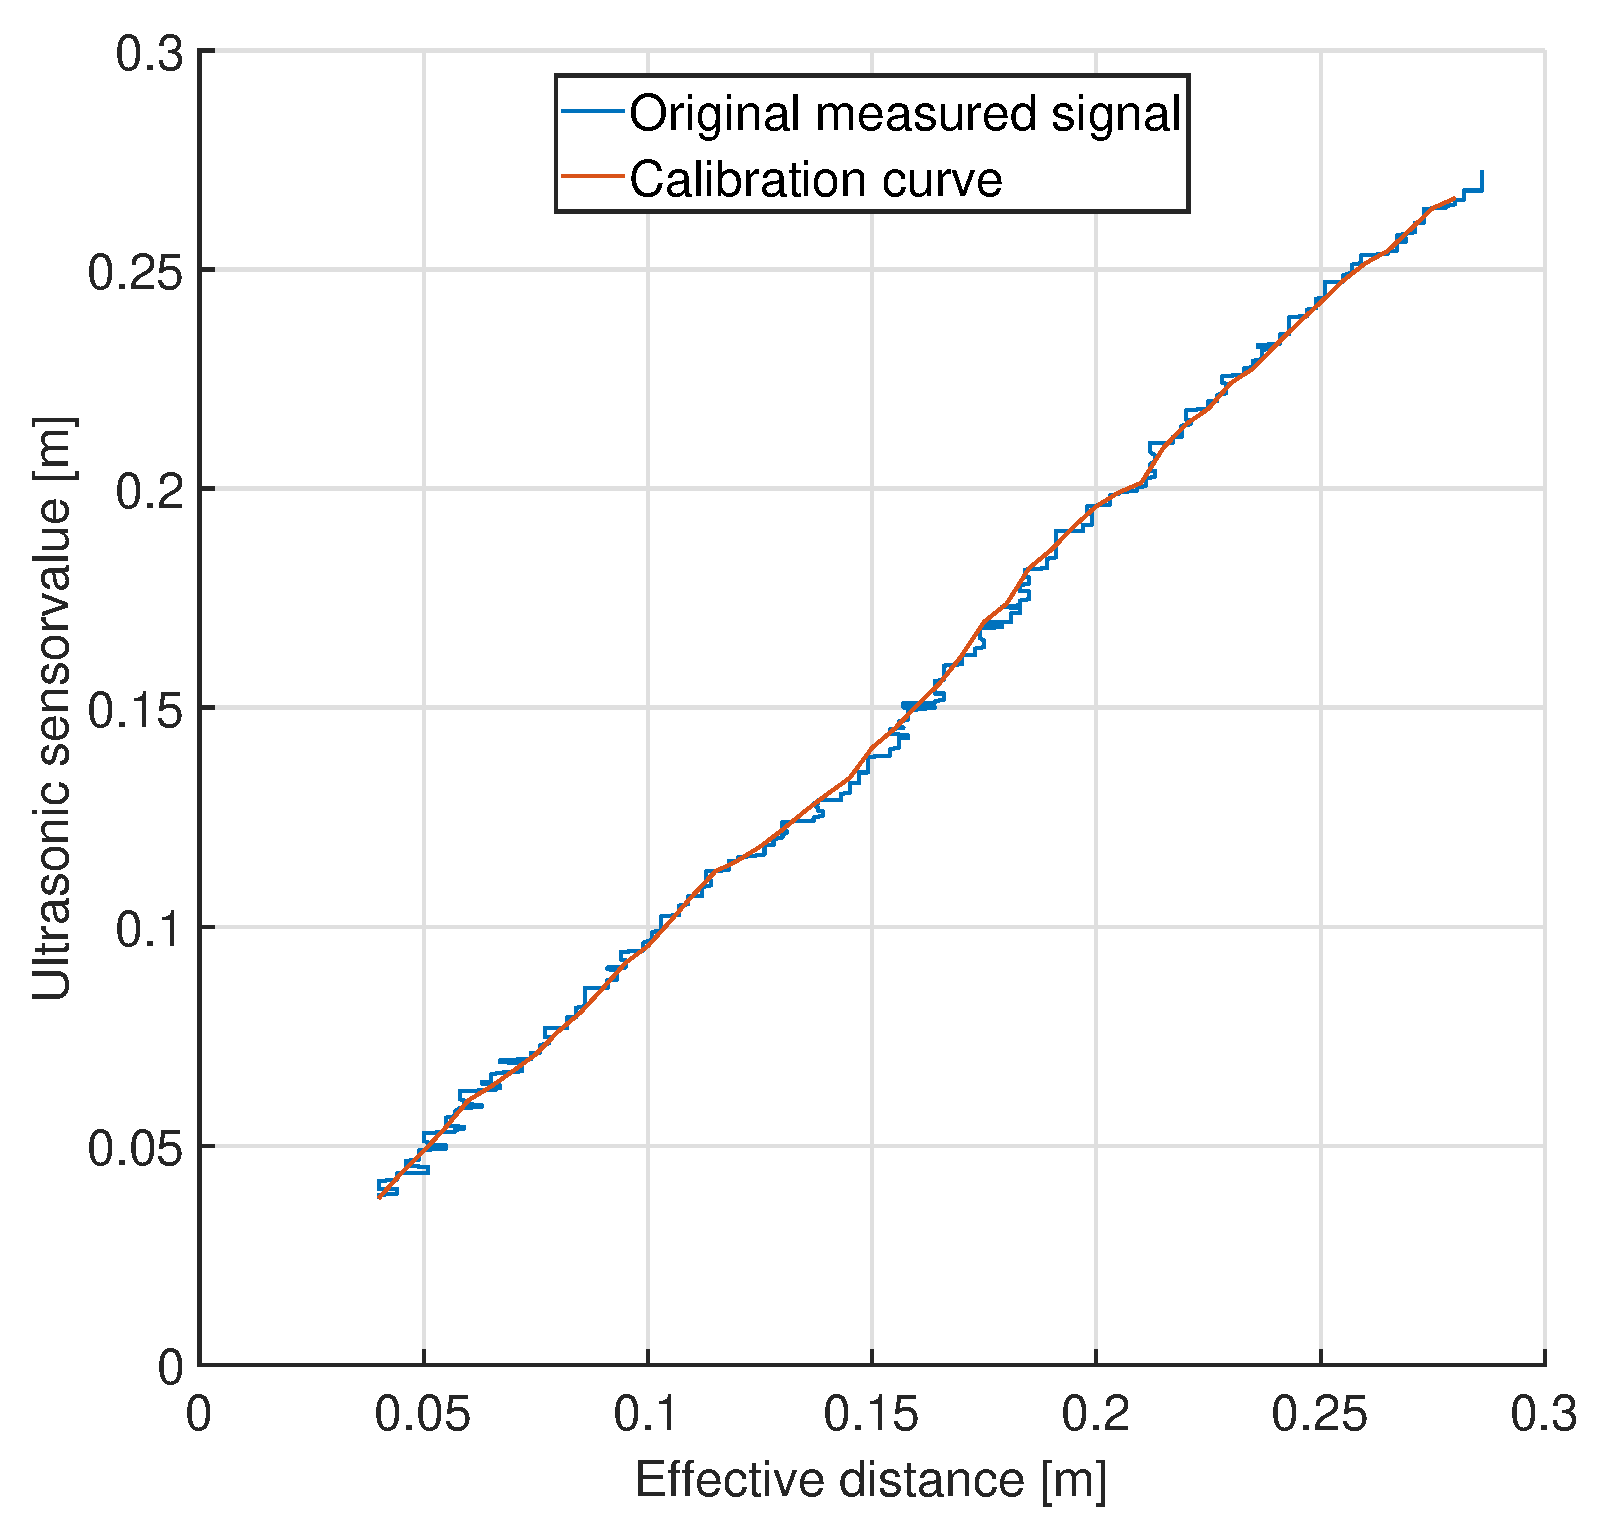
\includegraphics[keepaspectratio, width = 0.6 \textwidth]{Ultrasonic_CalibrationCurve_Dynamical.eps}
		\caption{Dynamical obtained calibration curve based on tachocounter and ultrasonic sensor values.}
		\label{fig:Ultrasoniccalibrationcurvedynamical}
	\end{figure}
	
	\par To investigate the dynamical behaviour of the sensor the internal motor tachocounter is used. When reducing the motor speed, the slipping of the tires can be assumed negligible. Therefore the sensorvalue can be plotted in function of the tachocounter value which represents the effective distance. Since the tachocounter is used as reference, a calibration curve for the sensor can be determined (Figure \ref{fig:Ultrasoniccalibrationcurvedynamical}). The obtained data is processed to obtain a strictly rising curve, which is necessary for lookup tables.
	
	\par The obtained calibration curve is used as lookup table in the software. Another problem is the probability of the non-linear curve. Hence, a moving average filter is implemented to cancel out stochastic noise. After the effort to stabilise the ultrasonic sensor, the implementation still doesn't satisfy the accuracy of positioning. 
	
	\par The implementation in the control software still confines the accurate performance. Drastically reduction of the speed could be a solution, since its deceleration time decreases drastically too. Hence, when the motor reaches its target position and his speed is low the motor could be stopped without making a large error. However, the position control keeps making a small error and the very slow speed is undesirable. These issues force to look for an alternative. During the tests, the tachocounter seems to be more reliable than first thought. Limiting the speed (not drastically) and smoothing the acceleration and deceleration provide negligible slip between the tires and the ground. Because of the internal tachocounter PID-controller and the negligible slip, the x-direction positioning is then reliable. Hence, a fusion of the tachocounter and the ultrasonic sensor is developed and implemented. The ultrasonic sensor will be used as homing and calibration reference for the tachocounter. In detail, the first riding sequence will be done using the above mentioned controlling strategy with the ultrasonic sensor. It's been tested that the ultrasonic sensor in its calibration range is reliable. Once its position is known, the tachocounter takes over. 
	
	\par Notice that the ultrasonic sensor could be replaced by some cheaper sensors such as a touch sensor against a wall or optical, capacitive or inductive sensors which are used a lot in industry. The latter can make use of a 2-directional homing sequence where first at high speed the robot goes towards its homing reference. Once it detects a rising software edge, it can go back slowly until it notices a falling edge. At the end, a very precise and efficient homing system can be used. These alternatives only show that simplification is possible, but the ultrasonic sensor is kept, because of the large effort therefore done.
	
	\par To ensure that the tachocounter based control holds its homing reference, an additional algorithm is foreseen. The robot moves between fixed stacking positions. Once he reaches a target position, the ultrasonic sensor could be used to check if the absolute distance equals more or less the estimated distance with respect to the tachocounter. If not, an additional correction parameter for the tachocounter will be tuned based on the measured error. Since the robot acts already reliable, the algorithm is foreseen but not activated in the code.
	
	\subsubsection{Vertical movement}
	\par Since the drive train consists of fixed connections and a gear-chain connection, no slip is present. Therefore the vertical measurement could also be replaced by position calculation based on the tachocounter. A homing sequence is necessary to determine its reference point. This could be executed by using a touch sensor (which is cheaper than an absolute distance sensor) or collision detection within the motor control. The latter proved its performance and is used consequently. Because in the early days of the project an ultrasonic sensor was installed for testing the y-direction, it is kept to support the homing sequence. The presence of the sensor ensures the gripper is at the predetermined position range when stalling.
	
	\par The height of the stacks will be detected by using a software edge detection based on the colour sensor and the y-direction height. This means the whole gripper should move up and down to calculate the height of each stack, which is a drawback of the upper gripper design. The algorithm to detect can be summerized as following:
	\begin{Verbatim}[fontsize=\small]
	Move down.
	
	If the coloursensor detects something:
	- calculate block level based on tachocounter
	- Go to the detected block level
	Return its level.
	\end{Verbatim}
	
	\subsubsection{Gripper}
	\par Also the gripper arms should have a positioning mode and in addition a torque control mode. The former will be used when the gripper is open, the latter when a block is clamped. Ideally also clamping could be performed by a positioning mode, but this never ensures the clamps to be closed enough. The torque control mode will be executed by using the standstill method of the available motor control software library. To home the gripper arms, this way of collision detection will be used too.
	
	\subsection{Colour-sensing}
	\par The obtained colour sensor has several working modes from which two directly related to colour-recognition. The first mode is the Colour-ID mode which translates a measurement into one integer which stands for a standard colour. The second mode is the RGB mode where the RGB values normalized with respect to 255 are returned. The former restricts the use of own selected colours and has no calibration method. Hence, the second mode is chosen, however the obtained RGB values strongly depend on environmental factors. A reliable solution is found and based on the invariance of the partial fraction of the RGB values with respect to the environmental conditions. The partial fractions are the normalizations of the measurements, such that a mutual RGB division remains:
	\begin{eqnarray}
	\left[R_{part} \; G_{part} \; B_{part}\right] = \frac{\left[R_{value} \; G_{value} \; B_{value}\right]}{\sqrt{R_{value}^2+G_{value}^2+B_{value}^2}}
	\end{eqnarray}
	with $X_{part}$ the normalized value and $X_{value}$ the sensor value.
	Figure \ref{fig:Calibration_ColourSensor} shows the proof by test measurements of this strategy. Obviously, the results of the normalized RGB vectors have a clear difference between several colours.
	\begin{figure}[H]
		\centering
		\includegraphics[keepaspectratio, width = 0.9\textwidth]{Figures/ColorSensor_Light_Dark_20180316.pdf}
		\caption{Test measurement of colour detection by RGB-mode (left: obtained sensor values scaled to 255, right: same measurement points but vector normalized).}
		\label{fig:Calibration_ColourSensor}
	\end{figure}
	\par The calibration of a colour itself is done by using a moving average algorithm which should be stabilised before accepting a new colour. After collecting all the necessary colours, the obtained calibration is written to a \textit{*.txt} file. The next time the robot will start-up it reads the file, such that directly stacking is possible. The user can at any point decide to force a new calibration sequence.
	
	\par The higher layer algorithm to identify the exposed colour consists of next decision steps. It's a combination of using fixed recognition ranges and estimating by relating the probability to the divergence.
	\begin{Verbatim}[fontsize=\small]
	If the sensor values are lower then a predetermined threshold:
	Return colour: None
	
	Check how many colours fall within a range in the vincinity of the calibrated colours
	- If there exists a unique one:
	Return that colour
	- If there are multiple:
	Return the best approximation by taking the sum of the separated R,G,B errors.
	
	If none of above
	Return colour: Unknown.
	\end{Verbatim}
	
	\section{Kinematics}
	\subsection{Motion representation}
	
	As mentioned in the description of the project, the positions of the blocks and pallet are known variables. For this, waypoints are defined to represent the different positions. A distinction is made between the translation of the robot and the gripper itself. First, we look at the motion of the system. The starting position, the three positions of the blocks and the pallet position gives five possible waypoints for the robot. An analogous reasoning can be used for the gripper.
	
	\subsection{Reference frame}
	
	
	
	
	The robot is modelled as a kinematic chain composed of two prismatic joint and an end effector. This modelling choice is applicable because of the nature of the robot actuation, which is composed of two sliding motions. The fixed coordinate system is placed at the starting position of the robot, as described in the mechanical design section. 
	
	The horizontal motion of the robot is modelled as the first prismatic joint, having its coordinate system at the base of the robot caterpillar track. The vertical motion of the gripper is modelled as the second prismatic joint and has its coordinate system at the base of the gripper. The reference frames, with x in horizontal and y in vertical direction, are illustrated in figure \ref{fig:framecoordinates}.
	
	\begin{figure}[H]
		\centering
		\includegraphics[keepaspectratio, width = 0.8\textwidth]{frame_coordinates.pdf}
		\caption{Reference frame of robot and gripper}
		\label{fig:framecoordinates}
	\end{figure}
	
	\subsection{Direct and inverse kinematics}
	
	Making use of the Denavit-Hartenberg formulation (slide 22, Kine2):
	\begin{align}
	g_{E}=g_{R} \cdot h_{RA} \cdot h_{AE}
	\label{eq1}
	\end{align}
	With $h_{RA}$ the transformation of the robot (first prismatic joint) and $h_{AE}$ the transformation of the gripper (second prismatic joint). These transformation matrices are expressed in the robot reference frame respectively the gripper reference frame. For this, we define $d_{1}$ as the translation along the x-axis expressed in the robot reference frame and $d_{2}$ as the translation along the y-axis expressed in the gripper reference frame. From this we obtain the transformation matrices:
	\begin{minipage}[t]{.33\textwidth-.5\columnsep}
		\centering
		\begin{eqnarray}
		h_{RA} = 
		\begin{bmatrix}
		1 & 0 & d_{1}\\
		0 & 1 & 0 \\
		0 & 0 & 1 \\
		\end{bmatrix} \nonumber
		\end{eqnarray}
	\end{minipage}%
	\begin{minipage}[t]{.33\textwidth-.5\columnsep}
		\centering
		\begin{eqnarray}
		h_{AE} = 
		\begin{bmatrix}
		1 & 0 & 0 \\
		0 & 1 & d_{2} \\
		0 & 0 & 1 \\
		\end{bmatrix} \nonumber
		\end{eqnarray}
	\end{minipage}
	\begin{minipage}[t]{.33\textwidth-.5\columnsep}
		\centering
		\begin{eqnarray}
		g_{E} = 
		\begin{bmatrix}
		1 & 0 & d_{1} \\
		0 & 1 & d_{2} \\
		0 & 0 & 1 \\
		\end{bmatrix} \nonumber
		\end{eqnarray}
	\end{minipage}\\
	Making use of slide 33:\\
	\begin{minipage}[t]{.33\textwidth-.5\columnsep}
		\centering
		\begin{eqnarray}
		s_{1} = 
		\begin{bmatrix}
		0 & 0 & d_{1} \\
		0 & 0 & 0 \\
		0 & 0 & 0 \\
		\end{bmatrix} \nonumber
		\end{eqnarray}
	\end{minipage}%
	\begin{minipage}[t]{.33\textwidth-.5\columnsep}
		\centering
		\begin{eqnarray}
		s_{2} = 
		\begin{bmatrix}
		0 & 0 & 0 \\
		0 & 0 & d_{2} \\
		0 & 0 & 0 \\
		\end{bmatrix} \nonumber
		\end{eqnarray}
	\end{minipage}
	\begin{minipage}[t]{.33\textwidth-.5\columnsep}
		\centering
		\begin{eqnarray}
		V = 
		\begin{bmatrix}
		v_1 \\
		v_2 \\
		\end{bmatrix} \vphantom{\begin{bmatrix} 0 \\ 0\\ 0\\ \end{bmatrix} } \nonumber
		\end{eqnarray}
	\end{minipage}\\
	
	\[
	\frac{d(g_{R}^{-1} \cdot g_{E} ) }{dt} = h_{RA} \cdot s_{1} \cdot h_{AE} \cdot v_{1} + h_{AE} \cdot h_{AE} \cdot s_{2} \cdot v_{2} = 
	\begin{bmatrix}
	0 & 0 & d_{1}\cdot v_{1}\\
	0 & 0 & d_{2}\cdot v_{2} \\
	0 & 0 & 0 \\
	\end{bmatrix}
	\]
	Since we don't need the whole configuration but only the translation of the gripper itself, the vector V can be obtained from this matrix. From the vector V, the matrix M can be calculated.
	
	\[
	\begin{bmatrix}
	d_{1} \cdot v_1 \\
	d_{2} \cdot v_2 
	\end{bmatrix}
	= M \cdot \begin{bmatrix}
	v_1 \\
	v_2 
	\end{bmatrix}
	\]
	
	The matrix M follows: 
	
	\[
	M = 
	\begin{bmatrix}
	d_{1} & 0 \\
	0 & d_{2} 
	\end{bmatrix}
	\]
	\begin{align}
	det (M) = d_{1} \cdot d_{2}
	\end{align}
	
	It follows that all movements are possible in the 2D space if both displacements $d_{1}$ and $d_{2}$ are not zero.
	
	
	
	\section{Software structure}
	\subsection{Blackboard}
	\par The ICT tasks are structured in a hierarchical decomposition. This has the advantage that the layers are programmed independently of each other. These tasks are: sense, plan, move, calibrate... The calibrating task is only executed at the start of the stacking. 
	\par Next to this, a blackboard is used to centralize some variables from the different layers. Every task can write and read from each global variable. The amount of global variables are reduced to the minimum. Firstly there is the state of the stacks, which keeps track of which block is where. Secondly there is the colour which holds the current colour that is sensed in enum format. Not the RGB-value because that has no meaning outside the task that colour-senses. In the same way the position is stored, but only the number of which stack it is at and which 'floor'. Because outside the move task, it doesn't matter which height each floor corresponds to. 
	\par The advantage is that since every task works independently, it is possible to make every task as general as possible, without having to care about how the information is used. If for example the colour-sensing task its implementation is changed, then the other task won't notice this since the colour-sensing tasks still just writes the colour in the agreed format to the blackboard. And thus other tasks don't have to change a single thing in there code.
	\par A schematic overview of the layers and the blackboard itself are given in figure \ref{fig:layers}. This structure carries also the advantage of easy implementation of threads. Since the layers only communicate by using the blackboard, threading has only to take care of the data-access.
	\par In figure \ref{fig:layers}, the \textit{position of the robot} by the ultrasonic sensor and the \textit{detected colour} by the colour sensor are straightforward. \textit{Current colour} indicates which colour block is being removed by the gripper. The remaining links given in the blackboard will be explained in the steering part.
	
	\begin{figure}[H]
		\centering
		\includegraphics[keepaspectratio, width=0.9\textwidth]{Figures/Layers_Blackboard.JPG}
		\caption{Layers and blackboard}
		\label{fig:layers}
	\end{figure}
	
	\subsection{Steering}
	The steering part deals with the basic movements of the gripper and the robot. As already explained, waypoints are used to define the positions for gripper and robot. These discrete positions are defined as an \textit{(enum)} type, \textit{stackPos} and \textit{heightPos} for respectively the horizontal position of the robot and the height of the gripper. The methods \textit{goToStack}, \textit{goToHeight}, \textit{openGripper}, \textit{closeGripper} are used for the basic movements of the robot and gripper. This explains the links in the blackboard, the status of both gripper and robot are updated by the steering part and used in the planning.  
	
	The ultrasonic sensor for the height measurement of the gripper was intentionally placed to work continuously in controlling the grip. As experiments have shown the measurement are quite unreliable in certain ranges. It should be noted that it is partly due to the small surface on which the ultrasonic wave is meant to reflect (see figure \ref{fig:Mechanical} backside of the caterpillar). As an alternative this ultrasonic sensor is only used during the homing of the gripper height. During which the gripper is driven to its uppermost height and the tachocounter reset to zero. This is done by steering it up until a motor stall is detected. To ensure that the stall is in fact the uppermost position, the ultrasonic sensor is used to measure that position.
	 As mentioned in previous section the ultrasonic sensor would ideally be left out and the calibration would rely only on the motor stall detection. However due to the rigidity of the caterpillar, a motor stall can sometimes be detected even if the gripper is not at it's uppermost height. After this homing sequence a fixed amount of rotation, which approximatively correspond to the height of one block, is used to move up and down. To make this movement more robust, the tachocounter of the motor is used, this allows to save the rotations of the motor while the colour sensor is used to detect the presence of any colour blocks. This is implemented in the method \textit{edgeDetect}, which is used in the first part of the stacking algorithm.
	
	At first, everything was implemented as it would function in a multithreading environment. However, everything was still sequential coupled. This way of implementation proves the functionality of the robot and allows easy debugging. At that time the robot succeeded in stacking blocks in a dynamical way, see later in planning. The following target was to optimise several stand-alone software components. The sensor data information gathering is successfully implemented in a separate thread. Steering and planning still run in the main thread. As will be mentioned in next sections, the higher algorithm is minimized in calculations, thus it will not affect the steering significantly. 
	
	\par In order to obtain a slightly smoother movement a kind of parallelism is introduced in the steering of the system. This is achieved by driving both the horizontal and vertical motor when lifting a block from one stack to another or leaving a stack after an \textit{edgeDetect}. This parallelism is obtained by starting
	the next movement a few moments before the current one ends. For example, when the gripper is moving up to a certain height, the movement in the horizontal direction will start as soon as the gripper height is in a certain range of it’s destination. This is illustrated in figure $ \ref{fig:parallellism} $. The same principle is used when going to a certain stack, the downwards movement will start as soon as the robot is in a certain range of the destination stack. 
	
	\begin{figure}[H]
		\centering
		\includegraphics[keepaspectratio, width = 0.7\textwidth]{Steering_Parallellism.pdf}
		\caption{Parallelism in steering ((red) followed trajectory, (blue) sequential trajectory)}
		\label{fig:parallellism}		
	\end{figure}
	
	
	\section{Planning}
	\subsection{Design process}
	\par This project requires a stacking algorithm that decides which steps are to be taken in order to reach the required stacking order.
	Our first thought for the design of the planning algorithm was to use dynamic optimization with cost-to-go functions. 
	The problem with that approach is the amount of calculation needed. In the case where there are 4 stacks and 4 blocks, each of these blocks can be placed on 3 other stacks at each step. Thus a total of 12 possible moves.  Assuming 10 steps are needed, then there are $12^{10}$ possible combinations. Of course this is a big overestimation, since calculating further on ineffective block placements isn't necessary and after a certain time there will be empty stacks which leads to less possible moves. The decision is made not to opt for the use of cost-to-go functions, striving for a general algorithm that can be applied for huge warehouses with much more blocks. 
	
	\par Instead a heuristic approach is chosen, which never looks in the future. Such an implementation is general, robust, very quick, and works for large warehouses.
	If we had to wait for the algorithm to load on the EV3 brick, and then wait for the robot to do the stacking, then debugging would be very slow. Secondly, testing many cases to make it robust would be very impractical.
	Therefore a virtual world was programmed that can do all the operations that the robot can do, while printing out a virtual representation of the robot. A small part of the sequence is shown in figure \ref{fig:stacking_sequence}.
	
	\par To implement this, we made a class Steering (which caries out the movement) with two subclasses: \textit{VirtualSteering} and \textit{LegoSteering}. 
	For example the commando \textit{moveTo(stack)} is implemented in \textit{LegoSteering} such that the robot physically goes to the intended stack, while in \textit{VirtualSteering} it is implemented such that it changes an internal virtual state which remembers that the gripper is now at that stack.
	So now in the main program, if we make the instance of steering an instance of the type \textit{LegoSteering}, the robot will execute the algorithm physically. While if it is an instance of \textit{VirtualSteering}, it will print out the order of execution of which a part is shown in figure \ref{fig:stacking_sequence}. Generating and printing this execution sequence only takes a very little amount of time.
	\begin{figure}[H]
		\centering
		\includegraphics[keepaspectratio, width=0.7\textwidth]{Figures/stacking_sequence.PNG}
		\caption{Part of a certain stacking sequence for 3 stacks}
		\label{fig:stacking_sequence}
	\end{figure}
	
	As a result, debugging is much faster and the design of more complicated heuristic methods is possible.
	This approach proved very helpful, since apart from some minor communicating errors, the planning algorithm worked immediately when trying to execute it physically.
	Also no extra effort is needed for all possible extras like for example more blocks, less stacks, stacks with no blocks, stacks with 4 blocks etc.
	This is because the heuristic method is made generally without specifying amount of blocks and stacks. Also the specified stack where the blocks need to be stacked can be changed.
	
	\subsection{Heuristic method}
	\par The heuristic methods consists of n steps, with n the number of blocks. 
	In each step, the goal of the algorithm is to place the current required block for stacking on the required stack and move the blocks that are in the way out of the way. The required stack is the stack on which all the block have to be placed in a predetermined order at the end of the algorithm. The current required block is the next block that needs to be placed on the required stack. The blocks are numbered from $0$ to $n-1$. Block $0$ is the block that needs to end on the bottom of the required stack, block 1 on top of that etc. In the following blocks will be referred to as higher and lower numbers, which means blocks with higher and lower numbers respectively (Not that they are placed higher or lower). For example if the required stack already consists out of the first two blocks (block $0$ and block $1$), then the current required block is the third block which has number two. It is obvious that $n$ steps are needed to finish the algorithm unless the required stack already contains some blocks in the right order at the start of the algorithm. 
	
	\par The stack of the current required block is called \textit{fromStack} and the stack of the required stack is called the \textit{goalStack} in figure \ref{fig:stacking_sequence}. The current required block is the block with number two, the \textit{fromStack} is the first stack and \textit{goalStack} is the third stack.
	
	\par To excecute a single step, firstly the algorithm tries to find all the blocks that are in the way (and thus have to be moved), called \textit{wrongBlocks}. These are the blocks that are above the current required block and blocks on the goal stack that shouldn't be there and should be moved such that the current required block can be placed on the \textit{goalStack}. In the stacking sequence in figure \ref{fig:stacking_sequence}, \textit{wrongBlocks} consists only of block $3$. Before the required block can be moved from the \textit{fromStack} to the \textit{goalStack}, it is required that the \textit{wrongBlocks} are placed on other stacks. These other stacks are called the auxiliary stacks or shortly \textit{auxStacks}. Thus each step of the algorithm can be divided in two main parts: firstly move all the blocks in \textit{wrongBlocks} out of the way and secondly move the current required block to the \textit{goalstack}. After this is done $n$ times, then the algorithm terminates.
	
	\par The second part of a step is obvious, only the first part needs to be explained. More precisely, where the \textit{wrongblocks} are placed and in what order. The placement of the \textit{wrongBlocks} is determined by a priority list of possible moves, this is explained in the next section. It is clear that the moves should be executed in such a way that the amount of future \textit{wrongBlocks} are minimised. Because then the amount of future moves is minimised.
	
	\par For each move of a certain \textit{wrongBlock}, the algorithm goes through a list of possible moves, called a priority list. The list is ordered according to priority. If for example the criterion for the move with priority \textit{p1} isn't met, then the move with priority \textit{p2} is checked. If the second criterion is met, then the second move will be executed and a certain \textit{wrongBlock} will be moved to a location decided by the second criterion. After that, the algorithm starts back again at the top of the priority list. This happens till all the \textit{wrongBlocks} are moved out of the way, such that the required block can be moved from the \textit{fromStack} to the \textit{goalStack}.
	
	\par A simplified version of the algorithm is shown in the following. A new scope is shown with a higher indentation level.
	
	\par
\begin{Verbatim}[fontsize=\small]
for each step:

 while the current step is not terminated, go through the priority list:

  update wrongBlocks.

  if no wrongBlocks left:                                                         (p1)     
   - Move required block from fromStack to goalStack.
   - The current step terminates.

  determine the highest wrongBlock that is on top of a stack, called the highestWrongBlock

  if there are empty auxStacks:                                                   (p2)                               
   - Move the highestWrongBlock to an empty auxStack.
   - Go back to top of the list.	

  if there is an auxStack whereof the block on top > highestWrongBlock:           (p3) 
   - Move highestWrongBlock to the auxStack of which the higher number is closest 
     (but bigger) to the number of the highestWrongBlock.
   - Go back to top of the list.
   - Move the highestWrongBlock to the auxStack whereof the minimum block number   
     is the highest.                                                              (p4)  

//The algorithm will never get here
\end{Verbatim}
	
	\par The reasoning behind this algorithm is that it is better to stack from high number to a low number on the auxiliary stacks (the stacks that are not the \textit{goalStack} and \textit{fromStack}), since low numbers need to be stacked first. 
	Otherwise if a block with a higher number was placed on top of a block with a lower number, then when the step comes that the current required block is that block with a lower number, an extra move is needed to move away the higher number that was placed on top, before the low number can be moved to the \textit{goalStack}. In other words, the latter case has an extra \textit{wrongBlock} in that certain step that could have been avoided. This is why the algorithm will move to the highest \textit{wrongBlock} from all the \textit{wrongBlocks} that are on top of a stack (called the \textit{highestWrongBlock}) if the first priority isn't met.
	
	\par The algorithm only places a higher on a lower number in the last element of the priority list (\textit{p4}). In that case, it prefers to stack on the stack with the highest minimum number, since that stack needs dismantling last. This is good, since that higher block won't be a \textit{wrongBlock} until it is really necessary. Otherwise it might be in a \textit{wrongBlock} for many steps. Which requires the block to be moved many times. An example follows.
	
	\subsection{Example}
	\par
	An example of a single step is given in figure \ref{fig:planning_example}. The respective numbers of the blocks are drawn on top. The required stacking order is red - green - blue - white as can be seen from the numbers. The \textit{goalStack} is set to the last stack. This is an example with only three stacks, because with 4 stacks usually only priority 1 and 2 are used. 
	\begin{figure}[H]
		\centering
		\includegraphics[keepaspectratio, width=1\textwidth]{Figures/planning_sequence.png}
		\caption{Example of planning sequence}
		\label{fig:planning_example}
	\end{figure}
	
	\par We start at (a) in the figure. The number of the step is 0, since the red block is not on the bottom of the \textit{goalStack}. Consequently, the current required block (the next block that is needed to be placed on the \textit{goalStack} as told before) is the red block (with number 0). The \textit{wrongBlocks} are in this case the red, green and blue block, since they are in the way at the \textit{goalStack}. Obviously the algorithm determines these \textit{wrongBlocks} automatically.
	
	\par
	Clearly, the first priority isn't met, so next the algorithm will go on to priority 2. The \textit{highestWrongBlock} is needed for all priorities from 2 onwards. Here there is only \textit{wrongBlock} on top of a stack, namely the red one. Thus the red block is the \textit{highestWrongblock} since there are no other \textit{wrongBlocks} on top of stacks with a higher number. 
	Priority 2 is met since there is an empty \textit{auxStack} (the second stack) and the robot will move the red block form the third to the second stack. Now we start back at the top of the priority list and the red block is removed from \textit{wrongBlocks}.
	
	\par
	Now we are in (b) in the figure. Notice that there now is only one \textit{auxStack}, namely the first one, since the second stack is the \textit{fromStack} (because the red block is now there) and since the third stack is the \textit{goalStack}. Priority 1 is still not met. The \textit{highestWrongBlock} is now block 1. The first priority that is met is priority 3. This is because there is an \textit{auxStack} whereof the top block has a higher number, namely the first stack has block 3 on top, which is a bigger number than the \textit{highestWrongBlock} (number 1). So block 1 is moved to the first stack.
	
	\par
	In (c), the \textit{highestWrongBlock} is block 2. The first priority that is met, is priority 4. There is one \textit{auxStack}, so block 2 will be placed there. 
	
	\par But to clarify the last priority, suppose that in (c) the second stack isn't the \textit{fromStack} (This might be the case when every block its number was increased by one and a new block 0 was placed somewhere else). In that case, the \textit{auxStacks} are the first and second stack. Block number 2 can thus be placed on both. In priority 4, the highest number of both stacks will be determined. This gives block 3 and 0 for the first and second stack respectively. The second stack has the lowest number and thus needs dismantling first in a later step. As a consequence, placing the blue block on the first stack will result in less \textit{wrongBlocks} in future steps.
	
	\par Now in (d) priority 1 is finally met since all \textit{wrongBlocks} are out of the way. The robot will move the red block to the \textit{goalStack}. 
	
	\par In (e), step 0 is terminated and step 1 will start. In this step block 1 will need to be placed on the third stack. It can be seen that the \textit{wrongBlocks} only consist out one block, namely block 2. Which will be placed on the \textit{auxStack} in priority 2. From then on only priority one moves are needed to finish the stacking. This shows the advantage of moving the \textit{wrongBlocks} in such a way that the future \textit{wrongBlocks} are minimised.
	
	\subsection{Footnotes}
	\par There is also a second algorithm for determining the positions of the blocks for when the robot is started up. First the colour and height of the top blocks of each stack are checked. Then blocks are moved out of the way on another stack if necessary to check the colour of the block(s) underneath. The algorithm tries to place those blocks that need to be moved away preferably on stacks of which the colours are already determined. Although it can also deal with situations where this is not possible, for example with seven blocks like in figure \ref{fig:stacking_sequence}. Also stacks without a block are possible.
	
	\par
	In an ideal case, an adapted method of the priority list is also used for determining the positions. In this way that stacking already happens while determining the positions. This methodology has been partly implemented, but contained in some unexpected cases a bug. Because this could not been tested extensively any more  to ensure the robustness of the algorithm, it is deactivated in the final program. In a warehouse application, the colour sensor should be able to determine the colours of all blocks, even if there are blocks on top. In that case, the extra algorithm is unnecessary, so this is more a compensation algorithm for our limiting mechanical design and is not deadly crucial.
	
	\par The gripper isn't steered to the highest height when it is not needed. It always leaves just enough space to travel without colliding with a stack of blocks. Unless in the beginning of the stack detection algorithm, because at that moment the heights of the stacks aren't known yet. Also sidetracking and moving up at the same time is implemented.
	
	\par The colour of the fourth block is still determined although the colour of that block can be known by appointing it the last colour. This is in line with our goal to make it as general as possible. Because there could be 5 blocks and thus more than four colours.
	
	\par The shortcoming of this algorithm is that the robot will never make a temporary bad move, which has good effect in the future. For example, it might be advantageous to move a low block to the \textit{goalStack} from an \textit{auxStack}, move a higher block to that \textit{auxStack} and finally move the high block back to that \textit{auxStack}. Such that the blocks are swapped compared to what would otherwise happen in priority 4. This is only efficient when the difference in the block number is at least 2. 
	
	
	\section{Conclusion}
	\par The objectives of our project included the stacking of four blocks, divided over three positions, on a pallet and the tower of Hanoi. 
	As a conclusion of our project, we can state that the proposed objectives are satisfied. 
	On the mechanical side, we provided some robustness by implementing more stability into the structure. During the test runs, some additional points of attention were revealed, such as the reliability of the ultrasonic sensor, some movements which could be executed more efficiently, etc. .
	The programming of the robot itself is implemented in a generic way, which is useful for small adaptations. These 
	adaptations can be for example changing the positions of the blocks.
	
	\par Since there is a full framework for the planning algorithm, it could be a successive project to implement, test for their performance and compare different stacking algorithms. This project only consists of making the framework and developing a self written, general but very robust, sorting algorithm.
	
	\section{Work distribution}
	The work was divided in 4 parts. 
	The first part is the only non-coding part. Shelly did this part. This part consists out of building the mechanical construction for the floor to guide the wheels as explained earlier. Lastly this part consists out of looking after the reports and see to it that the reports are good and cohesive.
	The second part consists out everything that is related to the kinematics of the robot. Namely the Denavit-Hartenberg transformations and also the control of each movement. This part was done by Ayoub and Fabrice. 
	The third part is the planning. In this part the algorithm for how to stack is written. This part is done by Jeroen.
	The last part is getting the sensor data and develop their calibrations. This is done by Gilke.
	
	\section{Movie}
	The results of the project can be consulted in a short video on youtube: \url{https://youtu.be/QX-tUiryg34}.
	
	
\end{document}